%% Use the hmcposter class with the thesis document-class option.
\documentclass[thesis]{hmcposter}
\usepackage{graphicx}
\usepackage{natbib}
\usepackage{booktabs}
\usepackage{subfig}
\usepackage{amsmath}
\usepackage{textcomp}
\usepackage{url}

\usepackage{hyperref}
\usepackage{cite}
\usepackage[utf8]{inputenc}
\usepackage[portuguese, english]{babel}

\usepackage{biblatex} 
\bibliography{refs}



%% Author of the thesis.
\author{Ayrton Denner da Silva Amaral}

%% The year of your thesis poster's creation.
\posteryear{2017}

%% Thesis Title.
\title{Predição de tendência de apostas em bolsas esportivas}

%% The name of the class for which the poster was created.
%% Generally we see posters for thesis and Clinic, but sometimes
%% other classes require or allow the creation of posters to
%% communicate the results of a project.
%% 
%% Use the format Math nnn: Class Title.
\class{Disciplina: Algoritmos de Reconhecimento de Padrões}

%% Advisor(s) name or names.  Separate with \and.
\advisor{Gustavo Teodoro Laureano\and Anderson da Silva Soares}

%% Reader(s) name or names.  Separate with \and.
%\reader{Gustavo Teodoro Laureano \and Anderson da Silva Soares}

%% Optional -- if you are especially concerned about intellectual
%% property issues (maybe you have some potentially patentable
%% material in your thesis), you can use the \copyrightholder
%% command to supply a name for a copyright holder for your
%% poster.  Note that under U.S. law, all works are under
%% copyright from the moment of creation; the copyright statement
%% is merely making your claim obvious.
%%
%% This command is also useful if you are sharing copyright of the
%% poster with someone else (e.g., a student collaborator, your
%% advisor, an organization).
%%
%\copyrightholder{Claire~M. Connelly and the Department of Mathematics, Harvey Mudd College}


%% Define the \BibTeX command, used in our example document.
\providecommand{\bibtex}{{\rmfamily B\kern-.05em%
    \textsc{i\kern-.025em b}\kern-.08em%
    T\kern-.1667em\lower.7ex\hbox{E}\kern-.125emX}}


\pagestyle{fancy}

\begin{document}

\begin{poster}

\section{Introdução}
% Note that we're not labeling sections because you shouldn't be
% doing a lot of referring back and forth in your poster---let the
% interested folks read your thesis or Clinic report, or ask
% questions.

Atualmente, a Betfair é a maior bolsa esportiva do mundo.
Com mais de 15 anos em atividade e 4 milhões de usuários cadastrados, movimenta aproximadamente £400 milhões anualmente. Na Figura~\ref{fig:betfair-print}, podemos ver uma imagem do site.

\begin{figure}
\begin{center}
\fbox{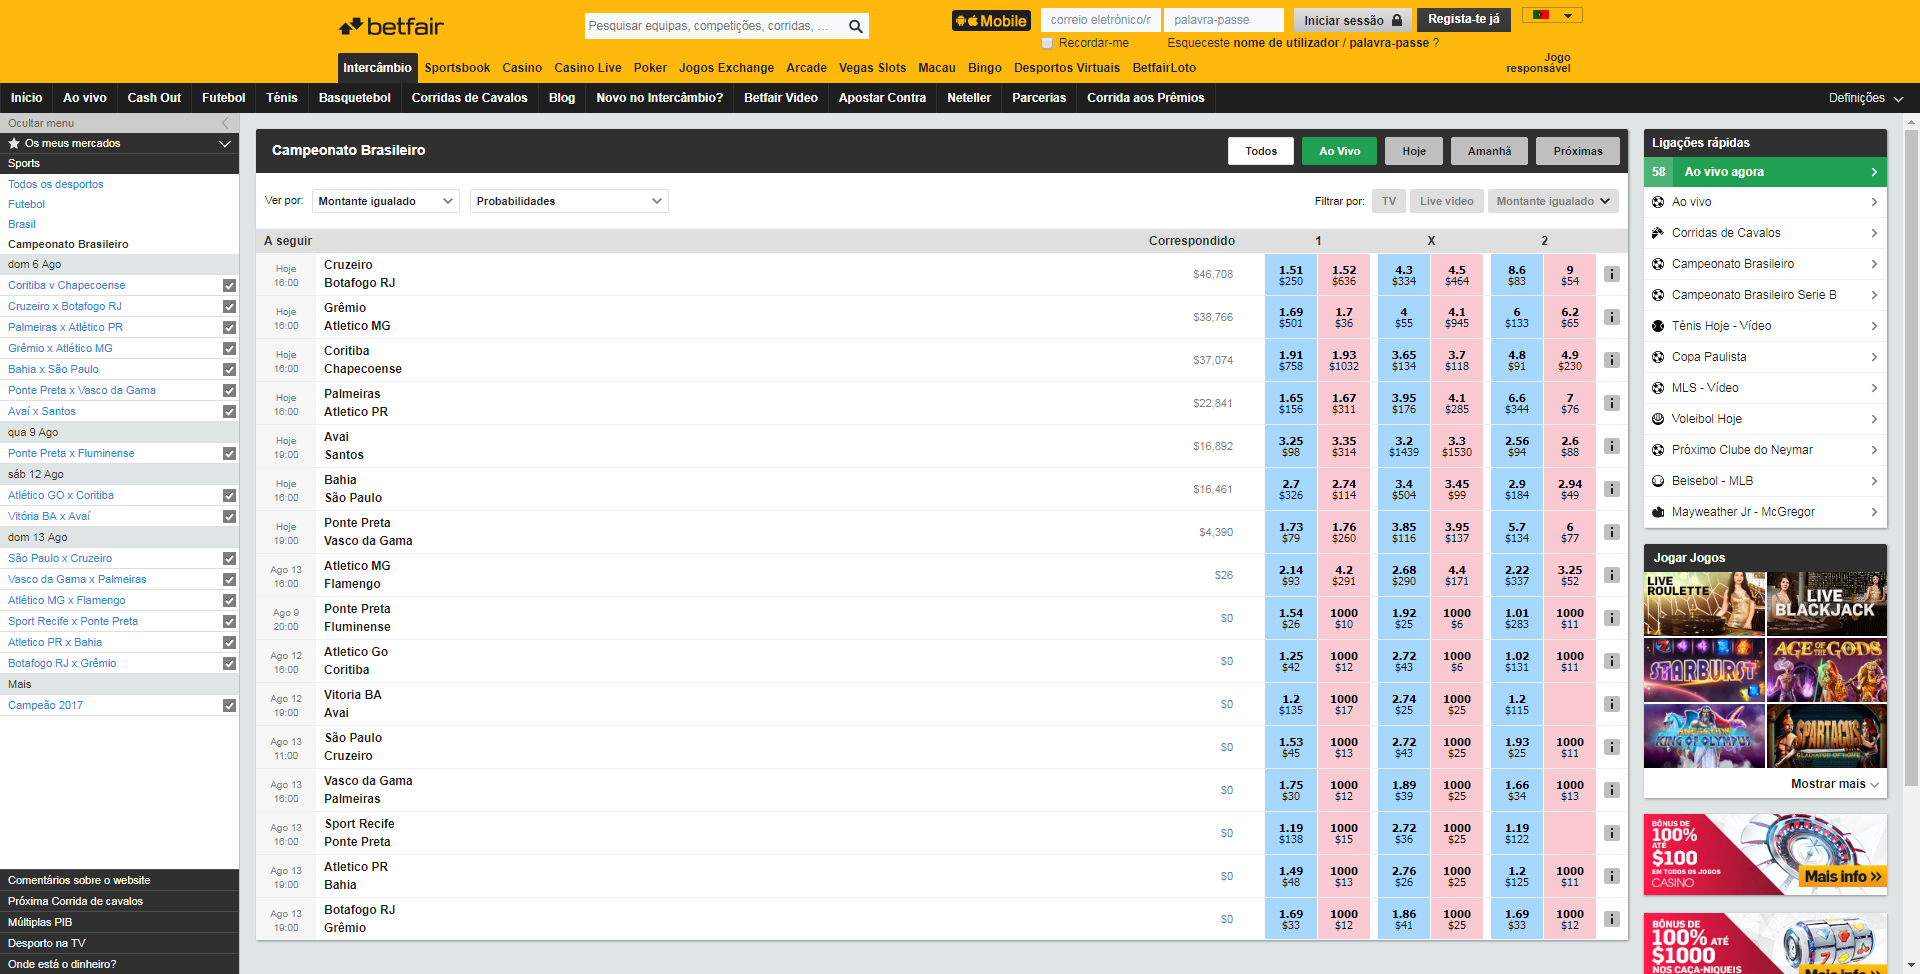
\includegraphics[width=10in]{screencapture-betfair-exchange-plus-football-competition-13-1502038892160.png}}
\caption{Imagem do site Betfair}%
\label{fig:betfair-print}
\end{center}
\end{figure}

Nesse projeto, buscamos a predição de qual categoria receberá um maior número de apostas em um período observado, seja o time da casa, time visitante ou opção de empate, analisando especificadamente os jogos da Série A do Campeonato Brasileiro de 2016.

\section{Materiais e métodos}%

Para o desenvolvimento do projeto, foram tomadas uma sequência de etapas para o uso dos dados:

\begin{itemize}
\item Foram utilizadas a biblioteca \emph{scikit-learn} para os algoritmos de aprendizado de máquina, e a biblioteca \emph{NumPy} para manipulação de vetores e matrizes, ambas utilizando a linguagem Python.
\item Também utilizamos a suíte \emph{Weka} para aplicação dos algoritmos de aprendizado de máquina.
\item Analisamos os dados oferecidos pela Betfair por todo o ano de 2016, em uma base de aproximadamente 55 milhões de linhas.
\item Ao aglutinarmos os dados de uma mesma partida, atingimos o número de 379 linhas, a mesma quantidade de jogos no ano de 2016.
\item Após filtramos as linhas necessárias para o estudo, foi necessário um pré-processamento dos dados oferecidos, como transformar datas e nome dos times em números (esse último via técnica de \emph{one-hot encoding}), e adicionar a quantidade de vitórias de cada time nos últimos 5 jogos.
\item No final de todas essas etapas, com todos os dados já preparados para o processamento, finalmente aplicamos os algoritmos de aprendizado de máquina de categorização aos valores obtidos.
\end{itemize}

\section{Resultados}%

Após filtramos e trabalharmos com os dados restantes, os primeiros resultados obtidos foram acerca da eficácia dos algoritmos preverem os resultados como um todo, exibidos na Figura~\ref{fig:total-algoritmo}:

\begin{figure}
\begin{center}
\fbox{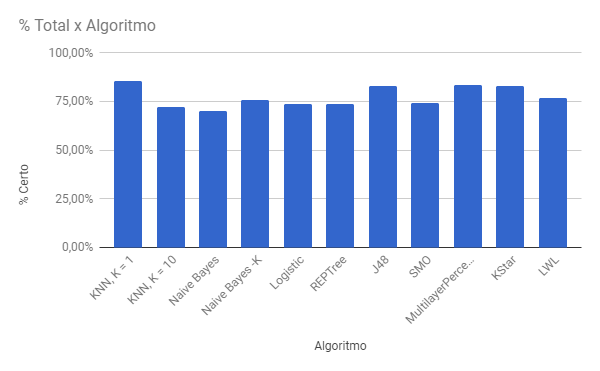
\includegraphics[width=10in]{imagens_algoritmo/total_algoritmo.png}}
\caption{Porcentagem de acerto dos algoritmos para todos os resultados}%
\label{fig:total-algoritmo}
\end{center}
\end{figure}

Porém, esses resultados não são suficientes. Por mais que os algoritmos tenham bons resultados com todos os valores, é necessário especificar a eficácia de cada algoritmo com cada categoria possível de resultado de apostas (time da casa, time visitante ou empate). Essa diferença se faz visível na próxima sequência da Figura~\ref{fig:casa-algoritmo}, Figura~\ref{fig:visitante-algoritmo} e Figura~\ref{fig:empate-algoritmo}:

\begin{figure}
\begin{center}
\fbox{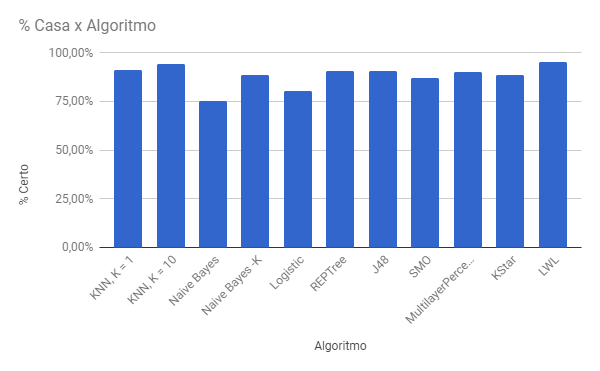
\includegraphics[width=10in]{imagens_algoritmo/casa_algoritmo.png}}
\caption{Porcentagem de acerto dos algoritmos para resultados com maioria de apostas do time da casa}%
\label{fig:casa-algoritmo}
\end{center}
\end{figure}

\begin{figure}
\begin{center}
\fbox{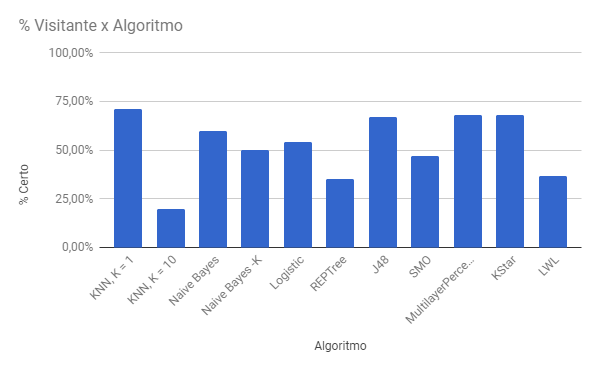
\includegraphics[width=10in]{imagens_algoritmo/visitante_algoritmo.png}}
\caption{Porcentagem de acerto dos algoritmos para resultados com maioria de apostas do time visitante}%
\label{fig:visitante-algoritmo}
\end{center}
\end{figure}

\begin{figure}
\begin{center}
\fbox{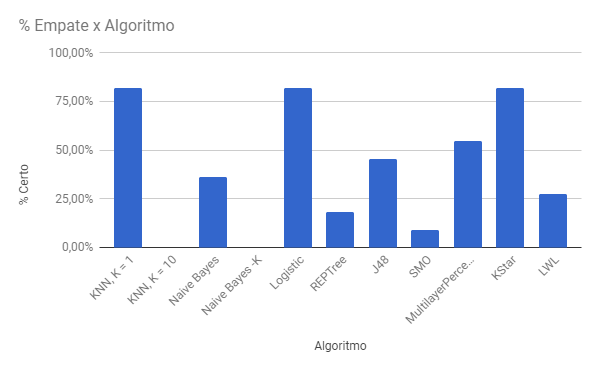
\includegraphics[width=10in]{imagens_algoritmo/empate_algoritmo.png}}
\caption{Porcentagem de acerto dos algoritmos para resultados com maioria de apostas do empate}%
\label{fig:empate-algoritmo}
\end{center}
\end{figure}

Com isso, é visível a diferença entre a análise dos valores como um todo, e a análise dos valores específicos de uma determinada classe. Outro valor utilizado para análise fora o chamado Coeficiente de Kappa. Tal coeficiente mede a concordância entre os valores da classificação apresentada, e o mesmo é representado na Figura~\ref{fig:kappa-algoritmo}:

\begin{figure}
\begin{center}
\fbox{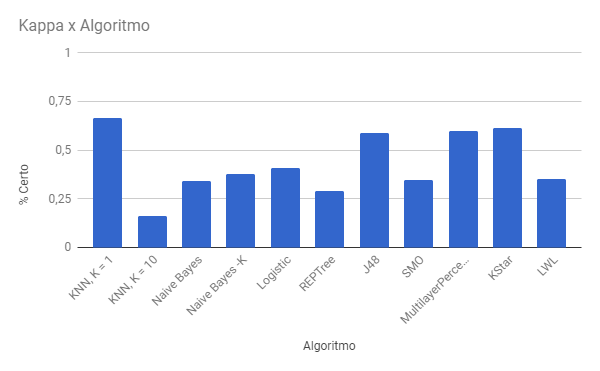
\includegraphics[width=10in]{imagens_algoritmo/kappa_algoritmo.png}}
\caption{Porcentagem do Coeficiente de Kappa para cada algoritmo utilizado}%
\label{fig:kappa-algoritmo}
\end{center}
\end{figure}

\section{Conclusões}

Ao final dessas análises, fica visível que um valor alto de acerto para o total de dados não é necessariamente um resultado bem-sucedido, podendo ser apenas um falso positivo que ignora a situação das categorias em específico.

Após esses resultados inicialmente positivos, o próximo passo para a predição de tendência de apostas é buscar não apenas a classificação, mas sim a quantificação de apostas em cada opção das bolsas esportivas. Ou seja, ao invés de utilizar algoritmos de classificação para indicar qual opção receberá mais apostas, utilizar algoritmos de regressão para indicar quantas apostas cada opção receberá.

Para a continuação das próximas etapas, faz-se necessário uma busca por bases mais completas em relação a eventos esportivos, com outros dados e estatísticas que possam melhor complementar a construção de um sistema de regressão de tendências.

% Force a column break here so the references begin the next column.
%\columnbreak

%% References.
%% Note that BibTeX will add its own section-level header, ``References''.

\section{Agradecimentos}

Por primeiro, gostaria de agradecer ao Instituto de Informática da Universidade Federal de Goiás, por dar apoio e ofertar disciplinas que, como essa, apoiam e fomentam a produção na comunidade e o estudo dos alunos.

Por segundo, gostaria de agradecer aos professores Anderson Soares e Gustavo Laureano, que ministraram a presente disciplina e também nos ajudaram na construção dos trabalhos e no entendimento do conteúdo apresentado.

Por terceiro, gostaria de agradecer aos colegas da disciplina de Algoritmos de Reconhecimento de Padrões, que também muito ajudaram no decorrer da disciplina o entendimento do conteúdo e também no incentivo do estudo dos tópicos apresentados

Por último, gostaria de agradecer a todos que ajudaram na construção desse conteúdo, e também daqueles que reservaram um pouco do seu tempo para prestigiar essa apresentação.

\section{Para maiores informações}

Possibly the most important section of your poster!  Tell people
how they can find out more about your research.  Be sure to
include
\begin{itemize}
\item Your e-mail address.  Mine's \url{cmc@math.hmc.edu}.
\item A URL for a website with more information.  \url{http://www.math.hmc.edu/computing/support/printing/posters/}.
\item If possible, a URL where they can download and read your full
  report.  The same as the last.
\item A URL where they can download your \emph{poster}.  And, again,
  the same URL will do you.
\end{itemize}

\cite{einstein}

%\section{Referências}

\printbibliography

%\bibliographystyle{ieee}
%\bibliographystyle{abbrv}

%\bibliographystyle{acm}
%\bibliography{biblio}

\end{poster}

\end{document}

 
